%!TEX root = ../../csuthesis_main.tex

\chapter{绪论}

本章主要介绍本课题研究的背景和意义,梳理国内外在行人强化学习控制与导航系统相关领域的研究现状,并简要概述论文的主要研究内容和技术路线。

\section{研究背景及意义}

近年来,随着人工智能技术和虚拟仿真平台的发展,基于强化学习的智能系统在自动驾驶与智慧交通领域得到了广泛应用。虚幻引擎(Unreal Engine)作为一款高性能仿真引擎,不仅提供了逼真的虚拟环境,还能生成多样化的模拟数据,为研究动态环境中的强化学习控制与导航问题提供了有效的实验平台~\cite{key1,key2}。

随着城市化进程的加速,智慧交通逐渐成为解决城市交通问题的关键手段。在自动驾驶技术的推广中,行人作为动态交通系统的重要参与者,其行为建模与智能化导航研究对提高交通效率与安全性具有重要意义~\cite{key3}。然而,当前智慧交通系统在动态场景下的行人行为预测与导航优化仍面临诸多挑战,例如复杂场景中多目标交互的实时性与准确性等。

虚拟仿真平台的快速发展为智能系统的研究提供了全新的手段。虚幻引擎以其高性能渲染和开放的二次开发能力成为构建虚拟实验环境的首选工具之一。通过结合强化学习技术,研究人员可以在仿真环境中生成大量高质量的实验数据,有效解决传统研究中实际场景数据获取困难的问题~\cite{key4}。本研究将虚幻引擎与强化学习方法相结合,旨在为复杂动态环境下的行人行为建模与导航优化提供新思路。

\section{国内外研究现状}

\subsection{行人行为建模}

行人行为建模是实现智能导航和行为控制的基础。传统方法多依赖于基于物理特征的步态建模和行为分析,例如通过人体运动学参数进行建模,但这些方法通常难以适应复杂场景的动态变化~\cite{key5,key6}。近年来,随着深度学习技术的发展,数据驱动的建模方法逐渐成为主流~\cite{key7}。

在国外,LSTM 模型被广泛应用于行人行为的时间序列预测中。例如,某些研究通过双向 LSTM 模型结合卷积网络,显著提高了行为建模的准确性~\cite{key8}。此外,基于 Transformer 的方法也开始应用于长序列建模任务,进一步提升了复杂行为的预测能力~\cite{key9}。

国内研究则更加注重复杂交通场景下的多目标交互,例如动态人群流动中的行为模拟和交通信号控制下的行人导航优化~\cite{key10}。尽管已有大量研究取得进展,但在高精度建模和复杂场景适应性方面仍有改进空间。

\subsection{行人导航技术}

行人导航技术是实现智能交通的重要组成部分。传统的行人导航方法主要基于惯性导航(PDR)或零速检测(ZUPT),这些方法通过分析行人的步长和航向实现路径规划。然而,这类方法对传感器性能要求较高,且在动态环境中的适应性较差~\cite{key11,key12}。

近年来,深度学习方法在行人导航领域取得了突破。例如,涂哲铭等提出了一种基于双向状态空间模型的行人导航算法,通过对时间序列惯性数据进行建模,显著抑制了误差漂移~\cite{key13}。此外,一些研究结合多传感器融合技术(如 GNSS 和 UWB),进一步提升了导航精度~\cite{key14}。

然而,在复杂的动态场景中,如何提高导航系统的实时性和鲁棒性仍然是研究的重点与难点。

\subsection{强化学习在行人控制中的应用}

强化学习因其在动态决策中的优越性能,近年来广泛应用于交通信号控制和路径规划中~\cite{key15}。基于强化学习的方法能够自适应复杂环境的动态变化,同时具备实时优化决策的能力。例如,陈飞等提出基于深度强化学习的行人过街信号控制模型,通过优先经验回放机制优化行人等待时间和车辆通行效率~\cite{key16}。

此外,多智能体强化学习方法近年来也受到关注。例如,在动态人群导航中,不同智能体之间的协作与竞争问题被引入到强化学习模型中,通过设计合理的奖励机制,显著提升了多目标场景中的决策效率~\cite{key17}。这些研究为本课题提供了重要的技术参考。

\section{本文研究内容及技术路线}

\subsection{研究内容}

本文主要研究基于虚幻引擎的行人强化学习控制与导航系统,研究目标包括:
\begin{itemize}
    \item 建立一个能够精确模拟行人行为的虚拟仿真环境,解决真实场景中实验成本高、数据获取难的问题;
    \item 提出一种基于深度学习的行人行为建模方法,通过分析骨骼运动数据实现对行人行为的准确预测;
    \item 利用强化学习优化行人导航策略,提升系统在复杂动态环境下的鲁棒性与适应性;
    \item 通过实验验证系统性能,探讨该方法在智慧交通领域中的应用潜力。
\end{itemize}

\subsection{技术路线}

本文的技术路线如图~\ref{fig:tech_route} 所示,具体步骤如下:
\begin{enumerate}
    \item \textbf{数据采集与处理}:通过虚幻引擎生成多场景行人数据集,包括骨骼运动数据和行为标签;
    \item \textbf{行人行为建模}:设计并训练深度学习模型(如 LSTM、Transformer)对骨骼数据进行建模;
    \item \textbf{强化学习控制系统设计}:基于 DQN 或 PPO 方法,优化复杂动态环境下的行人导航策略;
    \item \textbf{仿真实验与结果分析}:在虚拟仿真环境中测试系统性能,并与传统方法进行对比分析。
\end{enumerate}

\begin{figure}[htbp]
    \centering
    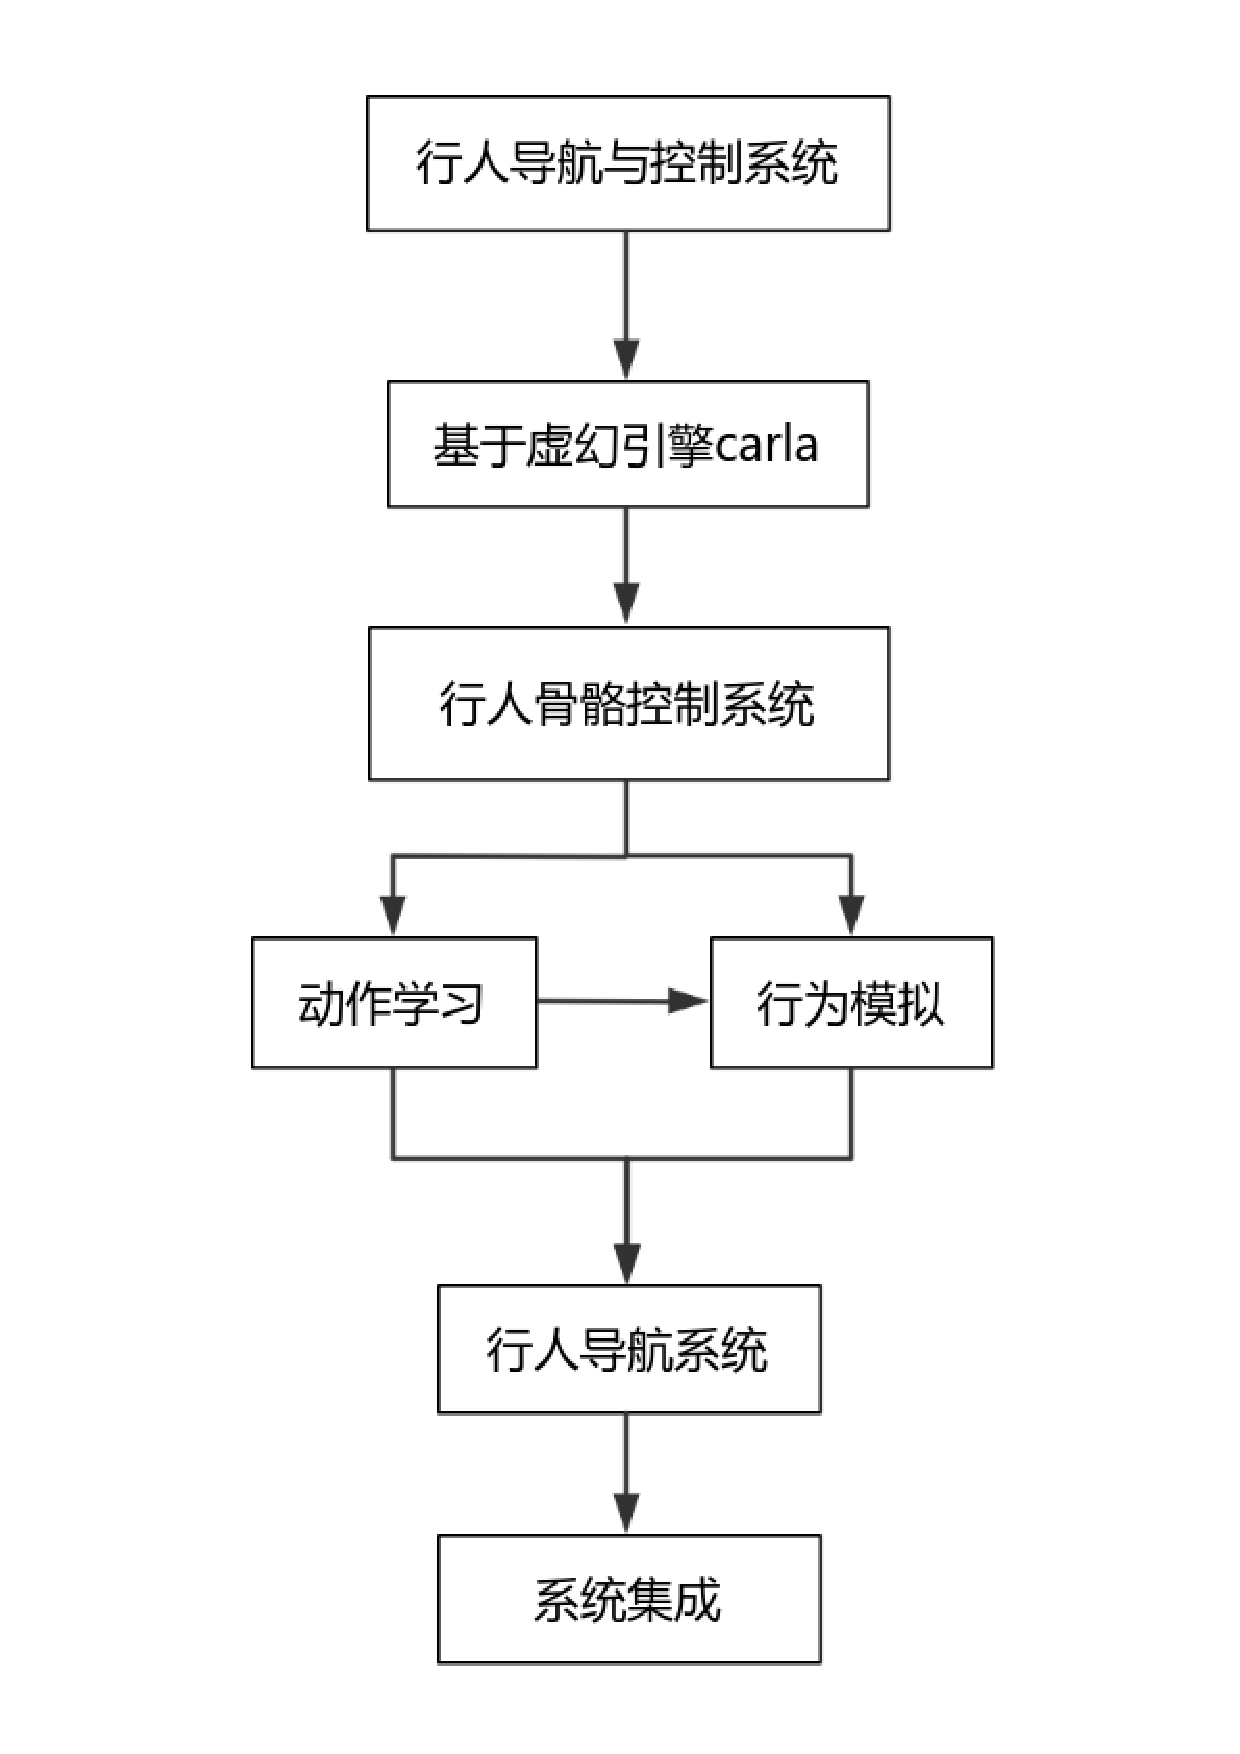
\includegraphics[width=0.8\textwidth]{tech_route.pdf}
    \caption{本文技术路线}
    \label{fig:tech_route}
\end{figure}
